%implementing document formatting:
\documentclass[a4paper,11pt,fleqn,dvipsnames,oneside,openright,oldfontcommands]{memoir} 	% Openright aabner kapitler paa hoejresider (openany begge)


%%%%%%%%% Indsat random
%makes it possible to refer to the name of a chapter rather than just the number.
\usepackage{nameref}
\usepackage{pdfpages}
\usepackage{marvosym}
\usepackage{setspace}
\usepackage{graphicx} % For at sætte 2 billeder ved siden af hinanden

%package for writing program code in latex
\usepackage{listings}
%%%%%%%%%%%%%%%%%%%%%%

% ¤¤ Oversaettelse og tegnsaetning ¤¤ %
\usepackage[T1]{fontenc}					% Output-indkodning af tegnsaet (T1)
\usepackage[danish]{babel}					% Dokumentets sprog
\usepackage[utf8]{inputenc}					% Input-indkodning af tegnsaet (UTF8)
\usepackage{ragged2e,anyfontsize}			% Justering af elementer
\usepackage{fixltx2e}						% Retter forskellige fejl i LaTeX-kernen							
				
																							
% ¤¤ Figurer og tabeller (floats) ¤¤ %
\usepackage{graphicx} 						% Haandtering af eksterne billeder (JPG, PNG, EPS, PDF)
%\usepackage{eso-pic}						% Tilfoej billedekommandoer paa hver side
%\usepackage{wrapfig}						% Indsaettelse af figurer omsvoebt af tekst. \begin{wrapfigure}{Placering}{Stoerrelse}
\usepackage{multirow}                		% Fletning af raekker og kolonner (\multicolumn og \multirow)
\usepackage{multicol}         	        	% Muliggoer output i spalter
\usepackage{rotating}						% Rotation af tekst med \begin{sideways}...\end{sideways}
\usepackage{colortbl} 						% Farver i tabeller (fx \columncolor og \rowcolor)
\usepackage{xcolor}							% Definer farver med \definecolor. Se mere: http://en.wikibooks.org/wiki/LaTeX/Colors
\usepackage{flafter}						% Soerger for at floats ikke optraeder i teksten foer deres reference
\let\newfloat\relax 						% Justering mellem float-pakken og memoir
\usepackage{float}							% Muliggoer eksakt placering af floats, f.eks. \begin{figure}[H]
\usepackage{array,booktabs,xcolor,longtable} % kan lave \hdashline i tabellertabe
\usepackage{arydshln}
\usepackage{tabu}

	
	
% ¤¤ Matematik mm. ¤¤
\usepackage{amsmath , amsthm , amsfonts , amssymb, float, stmaryrd} 		% Avancerede matematik-udvidelser
%\usepackage{mathtools}						% Andre matematik- og tegnudvidelser
\usepackage{textcomp}                 		% Symbol-udvidelser (f.eks. promille-tegn med \textperthousand )
\usepackage{rsphrase}						% Kemi-pakke til RS-saetninger, f.eks. \rsphrase{R1}
\usepackage[version=3]{mhchem} 				% Kemi-pakke til flot og let notation af formler, f.eks. \ce{Fe2O3}
\usepackage{siunitx}						% Flot og konsistent praesentation af tal og enheder med \si{enhed} og \SI{tal}{enhed}
\sisetup{output-decimal-marker = {,}}		% Opsaetning af \SI (DE for komma som decimalseparator) 

% ¤¤ Referencer og kilder ¤¤ %
\usepackage[danish]{varioref}				% Muliggoer bl.a. krydshenvisninger med sidetal (\vref)
\usepackage[numbers]{natbib}				% Udvidelse med naturvidenskabelige citationsmodeller
%\usepackage{xr}							% Referencer til eksternt dokument med \externaldocument{<NAVN>}
%\usepackage{glossaries}					% Terminologi- eller symbolliste (se mere i Daleifs Latex-bog)
\usepackage{lastpage}					% Gør det mulig at refere til sidste side 

% ¤¤ Misc. ¤¤ %
\usepackage{listings}						% Placer kildekode i dokumentet med \begin{lstlisting}...\end{lstlisting}
\usepackage{lipsum}							% Dummy text \lipsum[..]
\usepackage[shortlabels]{enumitem}			% Muliggoer enkelt konfiguration af lister
\usepackage{pdfpages}						% Goer det muligt at inkludere pdf-dokumenter med kommandoen \includepdf[pages={x-y}]{fil.pdf}	
\pdfoptionpdfminorversion=6					% Muliggoer inkludering af pdf dokumenter, af version 1.6 og hoejere
\pretolerance=2500 							% Justering af afstand mellem ord (hoejt tal, mindre orddeling og mere luft mellem ord)


% Kommentarer og rettelser med \fxnote. Med 'final' i stedet for 'draft' udloeser hver note en error i den faerdige rapport.
\usepackage[footnote,draft,danish,silent,nomargin]{fixme}		


%%%% CUSTOM SETTINGS %%%%

% ¤¤ Marginer ¤¤ %
\setlrmarginsandblock{3.0cm}{2.5cm}{*}		% \setlrmarginsandblock{Indbinding}{Kant}{Ratio}
\setulmarginsandblock{2.5cm}{3.0cm}{*}		% \setulmarginsandblock{Top}{Bund}{Ratio}
\checkandfixthelayout 						% Oversaetter vaerdier til brug for andre pakker

%	¤¤ Afsnitsformatering ¤¤ %
\setlength{\parindent}{6mm}           		% Stoerrelse af indryk
\setlength{\parskip}{0mm}          			% Afstand mellem afsnit ved brug af double Enter
\linespread{1,1}							% Linie afstand



% ¤¤ Indholdsfortegnelse ¤¤ %
\setsecnumdepth{subsection}		 			% Dybden af nummerede overkrifter (part/chapter/section/subsection)
\maxsecnumdepth{subsection}					% Dokumentklassens graense for nummereringsdybde
\settocdepth{section} 					% Dybden af indholdsfortegnelsen

% ¤¤ Lister ¤¤ %
\setlist{
  topsep=0pt,								% Vertikal afstand mellem tekst og listen
  itemsep=-1ex,								% Vertikal afstand mellem items
} 

%hyperlinks in the tabel of contents - comment this out before the report is printed.
\usepackage{hyperref}
\hypersetup{
	bookmarks = true,  % Show 'bookmark'-frame in pdf.
	colorlinks = true, % True = colored links, False = framed links.
	citecolor = black,  % Link color for references.
	linkcolor = black,  % Link color in table of contents.
	urlcolor = black,   % Link color for extern URLs.
}

% ¤¤ Opsaetning af figur- og tabeltekst ¤¤ %
\usepackage{caption}
%\usepackage{subcaption}
\captionnamefont{\small\bfseries\itshape}	% Opsaetning af tekstdelen ('Figur' eller 'Tabel')
\captiontitlefont{\small}					% Opsaetning af nummerering
\captiondelim{. }							% Seperator mellem nummerering og figurtekst
\hangcaption								% Venstrejusterer flere-liniers figurtekst under hinanden
%\captionwidth{0.9\textwidth}					% Bredden af figurteksten
\setlength{\belowcaptionskip}{0pt}			% Afstand under figurteksten
\captionsetup[figure]{labelfont={bf,it},font={it}} % sætter nummer til fed og kursis. Resten til fed + skriften er mindre end resten
\captionsetup[table]{labelfont={bf,it},font={it}} 


% ¤¤ Opsaetning af listings ¤¤ %

\definecolor{commentGreen}{RGB}{34,139,24}
\definecolor{stringPurple}{RGB}{208,76,239}

\lstset{language=Matlab,					% Sprog
	basicstyle=\ttfamily\scriptsize,		% Opsaetning af teksten
	keywords={for,if,while,else,elseif,		% Noegleord at fremhaeve
			  end,break,return,case,
			  switch,function},
	keywordstyle=\color{blue},				% Opsaetning af noegleord
	commentstyle=\color{commentGreen},		% Opsaetning af kommentarer
	stringstyle=\color{stringPurple},		% Opsaetning af strenge
	showstringspaces=false,					% Mellemrum i strenge enten vist eller blanke
	numbers=left, numberstyle=\tiny,		% Linjenumre
	extendedchars=true, 					% Tillader specielle karakterer
	columns=flexible,						% Kolonnejustering
	breaklines, breakatwhitespace=true,		% Bryd lange linjer
}

% ¤¤ Navngivning ¤¤ %
\addto\captionsdanish{
	\renewcommand\appendixname{Bilag}
	\renewcommand\contentsname{Indholdsfortegnelse}	
	\renewcommand\appendixpagename{Bilag}
	\renewcommand\appendixtocname{Bilag}
	\renewcommand\cftchaptername{\chaptername~}				% Skriver "Kapitel" foran kapitlerne i indholdsfortegnelsen
	\renewcommand\cftappendixname{\appendixname~}			% Skriver "Appendiks" foran appendiks i indholdsfortegnelsen
}

% ¤¤ Kapiteludssende ¤¤ %
%\definecolor{numbercolor}{gray}{0.7}		% Definerer en farve til brug til kapiteludseende
%\newif\ifchapternonum

\makechapterstyle{AAU}
{
	% Afstand mellem sidehovedet og kapitel+tal+kapitelnavnet defineres til:
	\setlength{\beforechapskip}{0cm}

	% Afstanden mellem kapitelnavnet og body-teksten defineres til:
	\setlength{\afterchapskip}{2cm}

	% Typografiopsætningen til kapitel+tal defineres til:
	\renewcommand\chapnamefont{\sffamily\bfseries\LARGE\raggedright}
	
	% Typografiopsætningen til kapitel+tal defineres til:
	\renewcommand\chaptitlefont{\sffamily\bfseries\huge\color[cmyk]{1.00,0.38,0.00,0.64}}

	% Forårsager, at der til kapitlet også tilføjes dets respektive tal:
	\renewcommand\chapternamenum{}
	\renewcommand\printchapternum
	{
		\makebox[0pt][l]
		{
			\color[cmyk]{1.00,0.38,0.00,0.64}
			\hspace{0.1cm}
			\resizebox{!}{1cm}{\chapnamefont\bfseries\sffamily\thechapter}
		}
	}
	
	% Definitionen af linjenstykket mellem ``Kapitel #'' samt ``kapitelnavnet'':
			\renewcommand\afterchaptertitle{\par\hspace{1.5cm}\hrule height 1pt\vskip\midchapskip}
}

% Aktivering af selve kapitellayoutet med dét navn, som definerer kapitellayoutet (ses fra tidligere):
\chapterstyle{AAU}

%\makechapterstyle{jenor}{					% Definerer kapiteludseende frem til ...
%  \renewcommand\beforechapskip{0pt}
%  \renewcommand\printchaptername{}
%  \renewcommand\printchapternum{}
% % \renewcommand\printchapternonum{\chapternonumtrue}
%  \renewcommand\chaptitlefont{\fontfamily{pbk}\fontseries{db}\fontshape{n}\fontsize{20}{25}\selectfont\raggedright}
%  \renewcommand\chapnumfont{\fontfamily{pbk}\fontseries{m}\fontshape{n}\fontsize{1in}{0in}\selectfont\color{numbercolor}}
% \renewcommand\printchaptertitle[1]{
%    \noindent
%    \ifchapternum
%     \begin{tabularx}{\textwidth}{XI}
%	{\let\\\newline\chaptitlefont ##1\par}     
%    \end{tabularx}
%    \par\vskip-2.5mm\hrule
%    \else
%    \begin{tabularx}{\textwidth}{X}
%      {\parbox[b]{\linewidth}{\chaptitlefont ##1}} & \raisebox{-15pt}{\chapnumfont \thechapter}
%    \end{tabularx}
%    \par\vskip2mm\hrule
%    \fi
%  }
%}											% ... her
%
%\chapterstyle{jenor}						% Valg af kapiteludseende - Google 'memoir chapter styles' for alternativer

% ¤¤ Sidehoved ¤¤ %

\makepagestyle{AAU}							% Definerer sidehoved og sidefod udseende frem til ...
\makepsmarks{AAU}{%
	\createmark{chapter}{left}{shownumber}{}{. \ }
	\createmark{section}{right}{shownumber}{}{. \ }
	\createplainmark{toc}{both}{\contentsname}
	\createplainmark{lof}{both}{\listfigurename}
	\createplainmark{lot}{both}{\listtablename}
	\createplainmark{bib}{both}{\bibname}
	\createplainmark{index}{both}{\indexname}
	\createplainmark{glossary}{both}{\glossaryname}
}
\nouppercaseheads											% Ingen Caps oenskes

\makeoddhead{AAU}{Gruppe 375}{}{\leftmark}				% Definerer lige siders sidehoved (\makeevenhead{Navn}{Venstre}{Center}{Hoejre})
\makeevenhead{AAU}{\rightmark}{}{Aalborg Universitet}		% Definerer ulige siders sidehoved (\makeoddhead{Navn}{Venstre}{Center}{Hoejre})
\makeevenfoot{AAU}{Side \thepage\ af \pageref{LastPage}}{}{}							% Definerer lige siders sidefod (\makeevenfoot{Navn}{Venstre}{Center}{Hoejre})
\makeoddfoot{AAU}{}{}{Side \thepage\ af \pageref{LastPage}}								% Definerer ulige siders sidefod (\makeoddfoot{Navn}{Venstre}{Center}{Hoejre})
\makeheadrule{AAU}{\textwidth}{0.5pt}						% Tilfoejer en streg under sidehovedets indhold
\makefootrule{AAU}{\textwidth}{0.5pt}{1mm}					% Tilfoejer en streg under sidefodens indhold

\copypagestyle{AAUchap}{AAU}								% Sidehoved for kapitelsider defineres som standardsider, men med blank sidehoved
\makeoddhead{AAUchap}{}{}{}
\makeevenhead{AAUchap}{}{}{}
\makeheadrule{AAUchap}{\textwidth}{0pt}
\aliaspagestyle{chapter}{AAUchap}							% Den ny style vaelges til at gaelde for chapters
															% ... her
															
\pagestyle{AAU}												% Valg af sidehoved og sidefod


%%%% CUSTOM COMMANDS %%%%

% ¤¤ Billede hack ¤¤ %
\newcommand{\figur}[4]{
		\begin{figure}[H] \centering
			\includegraphics[width=#1\textwidth]{billeder/#2}
			\caption{#3}\label{#4}
		\end{figure} 
}

% ¤¤ Specielle tegn ¤¤ %
\newcommand{\decC}{^{\circ}\text{C}}
\newcommand{\dec}{^{\circ}}
\newcommand{\m}{\cdot}


%%%% ORDDELING %%%%

\hyphenation{}

%%%%Fra engelsk til dansk i \autoref{•} %%%%
\renewcommand{\figureautorefname}{figur}
\renewcommand{\sectionautorefname}{afsnit}
\renewcommand{\subsectionautorefname}{afsnit}
\renewcommand{\subsubsectionautorefname}{afsnit}
\renewcommand{\tableautorefname}{tabel}
\renewcommand{\appendixautorefname}{bilag}
\renewcommand{\equationautorefname}{ligning}
\renewcommand{\itemautorefname}{punkt}
\renewcommand{\chapterautorefname}{kapitel}
%Figure references:
\newcommand{\figref}[1]{\textbf{figur \ref{#1}}}

%Figure references after full stop/period:
\newcommand{\Figref}[1]{\textbf{Figur \ref{#1}}}

%Table references:
\newcommand{\tableref}[1]{\textbf{tabel \ref{#1}}}

%Table references after full stop/period:
\newcommand{\Tableref}[1]{\textbf{Tabel \ref{#1}}}

%Units:
%inserting '\omit' before '{\put' prior ot final compile will fix allignment (and generate errors)
\newcommand{\unit}[1]{{\put(300,0){$\hfill\left[\: #1 \:\right]$}}}

%Text:
\newcommand{\tx}[1]{\text{#1}}

%Equation references:
%1 equation:
\renewcommand{\eqref}[1]{\textbf{ligning (\ref{#1})}}
%2 equations:
\newcommand{\eqrefTwo}[2]{\textbf{ligning (\ref{#1})} and \textbf{(\ref{#2})}}
%3 equations:
\newcommand{\eqrefThree}[3]{\textbf{ligning (\ref{#1})}, \textbf{(\ref{#2})} and \textbf{(\ref{#3})}}
%4 equations:
\newcommand{\eqrefFour}[4]{\textbf{ligning (\ref{#1})}, \textbf{(\ref{#2})}, \textbf{(\ref{#3})} and \textbf{(\ref{#4})}}
%5 equations:
\newcommand{\eqrefFive}[5]{\textbf{ligning (\ref{#1})}, \textbf{(\ref{#2})}, \textbf{(\ref{#3})}, \textbf{(\ref{#4})} and \textbf{(\ref{#5})}}
%5 equations:
\newcommand{\eqrefSix}[6]{\textbf{ligning (\ref{#1})}, \textbf{(\ref{#2})}, \textbf{(\ref{#3})}, \textbf{(\ref{#4})}, \textbf{(\ref{#5})} and \textbf{(\ref{#6})}}
%5 equations:
\newcommand{\eqrefSeven}[7]{\textbf{ligning (\ref{#1})}, \textbf{(\ref{#2})}, \textbf{(\ref{#3})}, \textbf{(\ref{#4})}, \textbf{(\ref{#5})}, \textbf{(\ref{#6})} and \textbf{(\ref{#7})}}

%Equation references after full stop/period:
%1 equation:
\newcommand{\Eqref}[1]{\textbf{Ligning (\ref{#1})}}
%2 equations:
\newcommand{\EqrefTwo}[2]{\textbf{Ligning (\ref{#1})} and \textbf{(\ref{#2})}}
%3 equations:
\newcommand{\EqrefThree}[3]{\textbf{Ligning (\ref{#1})}, \textbf{(\ref{#2})} and \textbf{(\ref{#3})}}
%4 equations:
\newcommand{\EqrefFour}[4]{\textbf{Ligning (\ref{#1})}, \textbf{(\ref{#2})}, \textbf{(\ref{#3})} and \textbf{(\ref{#4})}}
%5 equations:
\newcommand{\EqrefFive}[5]{\textbf{Ligning (\ref{#1})}, \textbf{(\ref{#2})}, \textbf{(\ref{#3})}, \textbf{(\ref{#4})} and \textbf{(\ref{#5})}}
%5 equations:
\newcommand{\EqrefSix}[6]{\textbf{Ligning (\ref{#1})}, \textbf{(\ref{#2})}, \textbf{(\ref{#3})}, \textbf{(\ref{#4})}, \textbf{(\ref{#5})} and \textbf{(\ref{#6})}}
%5 equations:
\newcommand{\EqrefSeven}[7]{\textbf{Ligning (\ref{#1})}, \textbf{(\ref{#2})}, \textbf{(\ref{#3})}, \textbf{(\ref{#4})}, \textbf{(\ref{#5})}, \textbf{(\ref{#6})} and \textbf{(\ref{#7})}}
\begin{document}

%||||||||||||||||||||||||||||||||||||||||||||||||||||||||||||||||
%|||||||				Example Inputs					 ||||||||
%||||||||||||||||||||||||||||||||||||||||||||||||||||||||||||||||
%|||||||												 ||||||||
%	\section{Figure Sample}

\begin{figure}[H]
	\caption{CAPTION\fxnote{Remember source}}
	\label{LABEL}
	\centering
	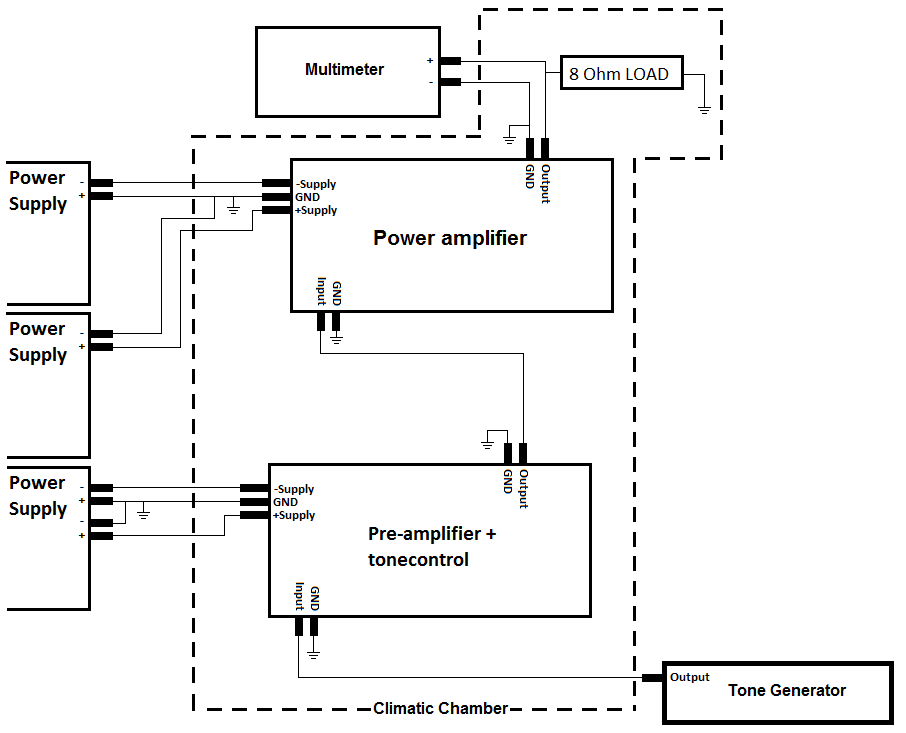
\includegraphics[scale=.8]{figures/filename}
	\flushleft
	\textit{SOURCE}
\end{figure}

%--------- NOTES ------------------------------------------------------
%Fxnotes wont compile properly inside the figure, only in the caption.
%Filetype can be specified but isn't needed.

\noindent
\figref{LABEL}\\

\noindent
\Figref{LABEL}

\vspace{.5cm}
%Do not use \vspace{length} or \hspace{length} unless exceedingly necessary.

%--------- BIBLIOGRAPHY REF EKSAMPLE -----------------------------------
This reference only represents this line since it is before the punctuation mark\cite{YDing}. This next reference however represents the entire section. That is all of the preceding sentences in the entire section. This is due to the fact that it is now after the punctuation mark in the end of the section (this is not used in the middle of a section!).\cite{YDing}
%>>>>>>>>>>>>>>>PLEASE ALSO READ THE NOTE IN myBib.bib<<<<<<<<<<<<<<<<<<
\pagebreak	%||||||||
%	\section{Table Sample}

\begin{table}[H]
\caption{This Is a Table\label{LABEL}}
\begin{tabular}{|l|p{5cm}|l|l|l|}
  \hline
  \textbf{No.}&\textbf{Description}&\textbf{Min}&\textbf{Max}&\textbf{Requirements}\\
  \hline
  1 & Some Text & Some Text & Some Text & Some Text\\
    &           &           &           & Some More Text\\
    &           &           &           & Text Text\\
    &           &           &           & Text Text Text\\
  \hline
  2 & Some Text & Some Text & Some Text & Some Text\\
  \hline
  3 & 	By specifying the width of a column (|p\{5cm\}|) the cells
  		in that column will will not exceed	the specified width    %Enter is used only for clarity and will not affect the compiled output.
  		but instead expand downward.
  		
  		        & Some Text & Some Text & Some Text\\
  \hline
  4 & Some Text & Some Text & Some Text & Some Text\\
  \hline
  \multicolumn{2}{|l|}{Some Text} 	&	\multicolumn{3}{l|}{Some Text}\\
  \hline
  \multicolumn{2}{|l|}{Text Text} 	&	\multicolumn{3}{l|}{Text = Text}\\
  \multicolumn{2}{|l|}{}			&	\multicolumn{3}{l|}{Text = Text}\\
  \multicolumn{2}{|l|}{}			&	\multicolumn{3}{l|}{Text = Text}\\
  \multicolumn{2}{|l|}{}			&	\multicolumn{3}{l|}{Text = Text}\\
  \multicolumn{2}{|l|}{}			&	\multicolumn{3}{l|}{Text = Text}\\
  \hline
  \multicolumn{2}{|l|}{Some Text} 	&	\multicolumn{3}{l|}{Teeeexxtt}\\
  \multicolumn{2}{|l|}{}			&	\multicolumn{3}{l|}{\LaTeX}\\
  \hline      
\end{tabular}
\end{table}

\noindent
\tableref{LABEL}\\

\noindent
\Tableref{LABEL}

\pagebreak	%||||||||
%	\section{Equation Sample}

\noindent
Some explanation:
%
\begin{align}
\unit{Unit}
[Equation]&=[Number]
\label{eq1}
\end{align}

\noindent
Some other explanation:
%
\begin{align}
\unit{Unit}
[Equation]&=[Number]
\label{eq2}
\end{align}

\noindent
Yet an explanation:
%
\begin{align}
\unit{Unit}
\text{You see? } [Equation]&=[Number]
\label{eq3}\\
%
\unit{Unit}
\text{Unit isn't aligned } \textbf{:( } \: [Equation]&=[Number]
\label{eq4}	   %
\end{align}	 	%
			  	 %
\noindent	   	  %
Explanation!:	   %
%				 	%
\begin{align}	  	 %
\unit{Unit}		   	  %
[Equation]&=[Number]   %	%-----------------------NOTES-----------------------%
\label{eq5}\\		 	%	% The &-sign aligns the equal signs.				%
%					  	 %	%													%
\unit{Unit}			   	  % % \unit{} will not be alligned by default,			%
[Equation]&=[Number]	   %% however the macro can be modded as described 		%
\label{eq6}\\			    % in macros.tex. This will allign the units,		%
%						    % but generate errors.								%
\unit{Unit}				    %													%
[Equation]&=[Number]		% \noindent should generally be used befor			%
\label{eq7}					% oneliners after equations, figures and tables.	%
\end{align}					%---------------------------------------------------%
\\
%
\noindent
\eqref{eq1}\\
\noindent
\eqrefTwo{eq1}{eq2}\\
\noindent
\eqrefThree{eq1}{eq2}{eq3}\\
\noindent
\eqrefFour{eq1}{eq2}{eq3}{eq4}\\
\noindent
\eqrefFive{eq1}{eq2}{eq3}{eq4}{eq5}\\
\noindent
\eqrefSix{eq1}{eq2}{eq3}{eq4}{eq5}{eq6}\\
\noindent
\eqrefSeven{eq1}{eq2}{eq3}{eq4}{eq5}{eq6}{eq7}\\
\noindent
\Eqref{eq1}\\
\noindent
\EqrefTwo{eq1}{eq2}\\
\noindent
\EqrefThree{eq1}{eq2}{eq3}\\
\noindent
\EqrefFour{eq1}{eq2}{eq3}{eq4}\\
\noindent
\EqrefFive{eq1}{eq2}{eq3}{eq4}{eq5}\\
\noindent
\EqrefSix{eq1}{eq2}{eq3}{eq4}{eq5}{eq6}\\
\noindent
\EqrefSeven{eq1}{eq2}{eq3}{eq4}{eq5}{eq6}{eq7}
\pagebreak	%||||||||
%|||||||												 ||||||||
%||||||||||||||||||||||||||||||||||||||||||||||||||||||||||||||||
%||||||||||||||||||||||||||||||||||||||||||||||||||||||||||||||||


%---------------------------INPUTS-------------------------------

%--------------------Introduktion--------------------------------
\chapter{Introduktion}

I dette kapitel beskrives udførte test på den analoge og digitale del af systemet. Hertil undersøges de forskellige delelementer af systemet, og om de opstillede krav overholdes. Måden hvorpå testen generelt vil blive udført, er ved at anvende kontrolleret data (målinger fra pilotforsøget), og efterfølgende undersøge om den testede systemdel udføre den tiltænkte funktion. 

  
\input{rapportAfsnit/bInitierende/initierende_spg.tex}

%-----------------------Problemanalyse---------------------------
\chapter{Problemanalyse}
\section{Amyotrofisk lateral sklerose} \label{sec:ALS}
ALS er en neurodegenerativ sygdom, der påvirker motorneuronerne i hjernen, hjernestammen og rygsøjlen i takt med sygdommens fremskriden, hvilket resulterer i muskelsvaghed \citep{henschke2012}. 
En illustration af, hvordan ALS påvirker motorneuroner, illustreres på \autoref{fig:affectedneuron}. 
De første symptomer på sygdommen er kramper, svaghed samt stive muskler, hvilket kan opstå som muskelsvaghed i arme eller ben, talebesvær eller svaghed i de muskler, som styrer respirationen \citep{nationalinstitute2016}. 
Symptomer og følger af ALS varierer fra patient til patient, hvorved nogle patienter først oplever muskelsvaghed i deres ben, mens andre oplever muskelsvaghed i deres hænder og arme eller besvær ved tale- eller synkebesvær \citep{nationalinstitute2016, miller2005}.

\begin{figure}[H]
\centering
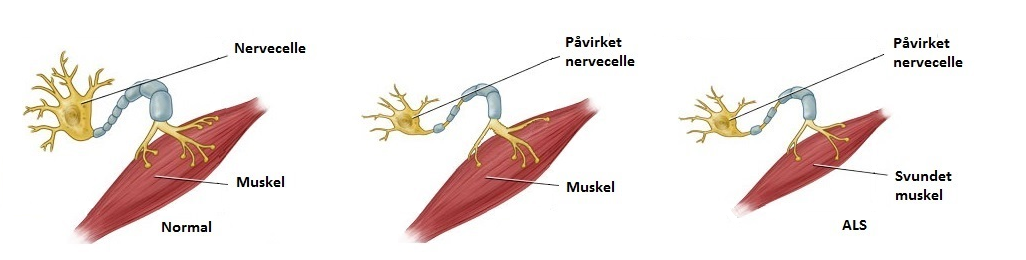
\includegraphics[width=1\textwidth]{figures/affectedneuron}
\caption{Nervecelle og muskel påvirket af ALS. Til venstre ses en normal motorneuron samt en upåvirket muskel. I midten fremgår motorneuronet påvirket af ALS, dog ses musklen endvidere upåvirket. Til højre ses motorneuronet påvirket, samt at musklen er svundet ind. Svindet skyldes en manglende stimulering af musklen som følge af den påvirkede motorneuron \citep{drake2015}.}
\label{fig:affectedneuron}
\end{figure}
 
\noindent
Muskelsvagheden skyldes abnormiteter i de nedre motorneuroner. De nedre motorneuroner er de nerveceller, der videregiver information fra rygmarven til musklerne. 
Symptomer på abnormiteter i de nedre motorneuroner ses som muskelsvaghed samt muskelkramper og atrofi.
Ligeledes kan de øvre motorneuroner påvirkes. Disse motorneuroner sørger for kommunikationen mellem hjernen og de nedre motorneuroner i rygmarven. 
Ved abnormitet, opstår komplikationer ved vidersendelse af beskeder til det givne sted. 
Dette ses som spasticitet samt overdrevne reflekser \citep{nationalinstitute2016}. Opdelingen af de nedre samt øvre motorneuroner ses på \autoref{fig:motorneuroner}.

\begin{figure}[H]
\centering
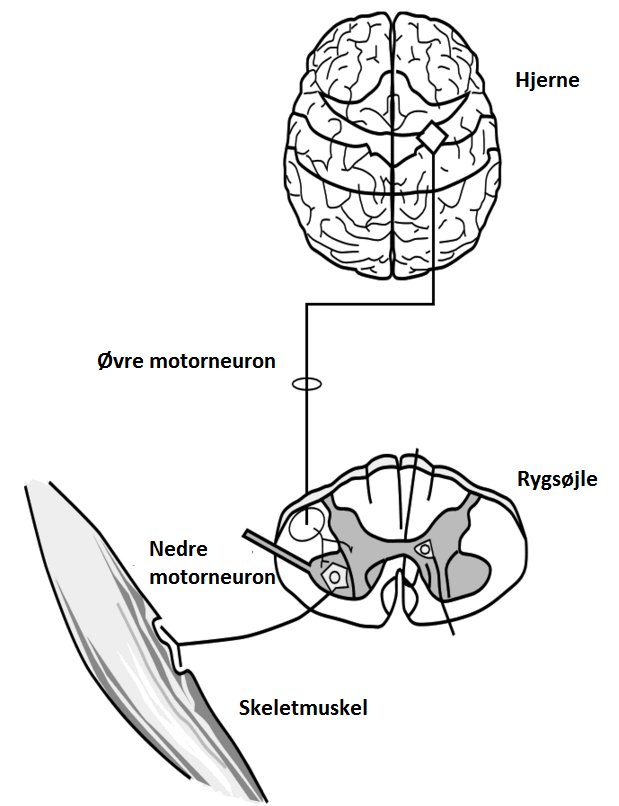
\includegraphics[width=0.6\textwidth]{figures/motorneuroner.png}
\caption{Illustrerer opdelingen af de nedre samt øvre motorneuroner i forhold til hjernen, rygsøjlen og skeletmuskulaturen \citep{miller2005}.}
\label{fig:motorneuroner}
\end{figure}

\noindent
Årsagen til ALS' opståen er oftest ukendt, dog ses en arvelighed i $5 - 10~\%$ af tilfældene. Heraf anslås, at $20~\%$ har det muterede Superocide dismutase 1-gen (SOD-1), hvilket resulterer i tab af motorneuroner \citep{miller2005}.

På trods af, at ALS opleves individuelt både i forhold til sygdomsprogressionen samt, hvilke komplikationer de oplever, kan sygdommen inddeles i tre stadier: et tidligt, midt og endeligt stadie. Et diagram af de tre stadier fremgår af \autoref{fig:stadier}.

\begin{figure}[H]
\centering
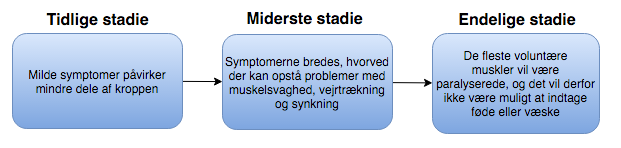
\includegraphics[width=1\textwidth]{figures/stadier.png}
\caption{Tre stadier for udviklingen af ALS samt de tilhørende symptomer.}
\label{fig:stadier}
\end{figure}

\noindent
I det tidlige stadie kan patienter overse symptomer på ALS, da disse er milde og kun påvirker mindre dele af kroppen \citep{themusculardystrophyassociation2016}. 
Ved det midterste stadie vil symptomerne udbrede sig, og nogle muskler paralyseres. Andre muskler vil blive svagere med tiden, hvilket blandt andet kan medføre problemer med synkning og vejrtrækningen \citep{themusculardystrophyassociation2016}. I det endelige stadie vil de fleste voluntære muskler være paralyserede, og det vil derfor forringe muligheden for selv at indtage føde eller væske. 
Herudover vil patienter oftest i dette stadie miste evnen til selv at trække vejret, og de bliver derfor afhængige af ventilationsstøtte \citep{themusculardystrophyassociation2016}.
Den mest almindelige dødsårsag er respirationssvigt, hvilket oftest sker inden for tre til fem år efter diagnosen er stillet \citep{morris2015}. $25~\%$ af patienterne har en overlevelsesrate på fem år, og kun $10~\%$ lever længere end ti år efter diagnosen er stillet \citep{grehl2011, miller2005}.


%Til at starte med kan mindre symptomer som besvær ved at gå op ad trapper opstå. Ligeledes kan patienterne være påvirket af dropfod, når de går. Herefter vil musklerne gradvist blive svagere, og med tiden vil patienterne ikke længere være i stand til at gå.\citep{tidy2015} 
% !TeX spellcheck = da_DK
\subsection{Følger af amyotrofisk lateral sklerose}
..... Skriv noget her ...
% !TeX spellcheck = da_DK
\subsection{Nuværende teknologier/hjælpemidler}
% Da der ikke er nogen bevis kur for ALS er teknologierne er pallialiv, dvs. at den er lindrende. 
Som tidligere nævnt er ALS en livstruende sygdom, hvor følgerne sker gradvist, hvilket gør at patienternes funktionelle evner svækkes over sigt, hvorfor der er behov for en række hjælpemidler som helt eller delvist kan være en hjælp i hverdagen. Nogle af hjælpemidlerne er i starten af sygdommen for at patienterne kan klare sig selvstændigt, hvor der senere er behov for andre hjælpemidler samt helt eller delvist hjælp fra en ægtefælde eller plejepersonale. Der anvendes på nuværende tidspunkt teknologiske og personlige hjælpemidler. [2]

\subsubsection{Teknologiske og personlige hjælpemidler}
De mest anvendte hjælpemidler for patienter med ALS er teknologiske som f.eks.  kørestole, toiletstole og stokke. Hjælpemidlerne er alle redskaber som støtter og aflaster patienten. Derudover anvendes der mere personlige hjælpemidler som i stedet er tilpasset patienterne individuelt. Patienterne har på denne måde et særligt behov for hjælpemidler som f.eks. tilpasset kørestole, tilpasset fodtøj og høreapparat. [2]

\subsubsection{Udfordringer og muligheder}
\fxnote{På nuværende tidspunkt har det være svært at finde nogle kilder i forhold til muskelsvind og det at gå, men mine tanker er noget med at koble det sammen ift. det der står under livskvalitet og de nuværende teknologier der er hvor lidt selvstændighed det giver i hverdagen og så senere koble det til at kunne anvendes exoskelet........}
Der er ingen af de nuværende teknologier som giver patienten mulighed for at gå, men hvis patienterne har gangbesvær vil de kunne anvende hjælpemidler som stok og rollator, ellers vil de være nødsaget til at anvende en kørestol for at kunne komme fra A til B. hvilket i forhold til livskvalitet bla..bla..blaa.. er patienterne gerne vil gå.


\subsubsection{Løsning}
Exoskelet som har til opgave at......




Det er her udover påvist at flere af disse metoder ud fra patienternes vurdering medvirker til en forbedret livskvalitet [1]

%[1] http://www.tandfonline.com.zorac.aub.aau.dk/doi/pdf/10.1080/00222895.2014.891970
%[2] https://books.google.dk/books?id=ha23lFiOGX8C&printsec=frontcover&hl=da&source=gbs_vpt_buy#v=onepage&q&f=false Grundbog om hjælpemidler - til personer med funktionsnedsættelse Åse brandt og lilly Jensen 
% !TeX spellcheck = da_DK
\section{Gangfunktion}
Efterhånden som ALS-patienter mister muskelkraft, vil bevægeligheden i deres led nedsættes. Af denne grund opstår der kontrakturer i led, og muskelstramninger i de omkringliggende muskler.

Ved gang anvendes knæ-, hofte- og ankelleddet, hvilket fremgår af \autoref{fig:knaet}, hvis disse led ikke akviteres, opstår der muskelstramninger i benene \citep{instforms2008}.

\begin{figure} [H]
\centering
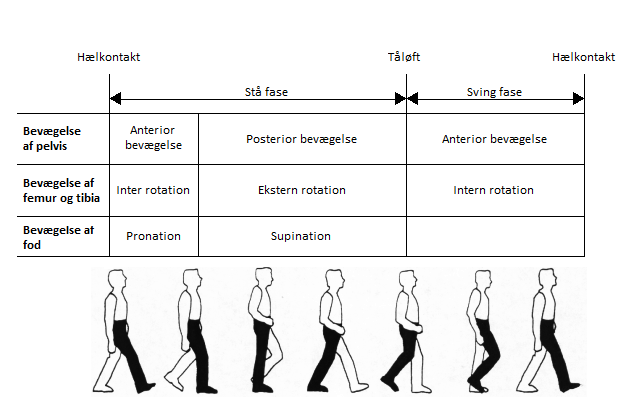
\includegraphics[width=0.9\textwidth]{figures/knaet}
\caption{Viser bevægelse af pelvis, femur og tibia samt foden ved forskellige faser under gang \citep{orthopedics2016}.}
\label{fig:knaet}
\end{figure} 

\noindent
Knæleddet vælges som udgangspunkt for et muligt body augmentation-system i form af et exoskelet, da knæleddet er et hængselled og derfor har et begrænset antal frihedsgrader. Knæleddet har én frihedsgrad, modsat andre mere komplekse led, hvilket gør, at leddet kun kan bevæge sig i én akse \citep{martini2012}. 
Det antages derfor, at knæleddet er et af de led, som er simplest at opbygge et system omkring. 
Hvis der kan laves et exoskelet omkring knæleddet, vil det kunne antages, at samme princip kan muliggøres ved henholdsvis hofte- og ankelleddet, hvorved gangfunktionen kan opretholdes.

\subsection{Knæets opbygning}
Knæet består af tre separate ledforbindelser. To, der er forbundet mellem femur og tibia, samt en mellem patella og femur, hvilket fremgår af \autoref{fig:knae_anatomi}. 

\begin{figure}[H]
\centering
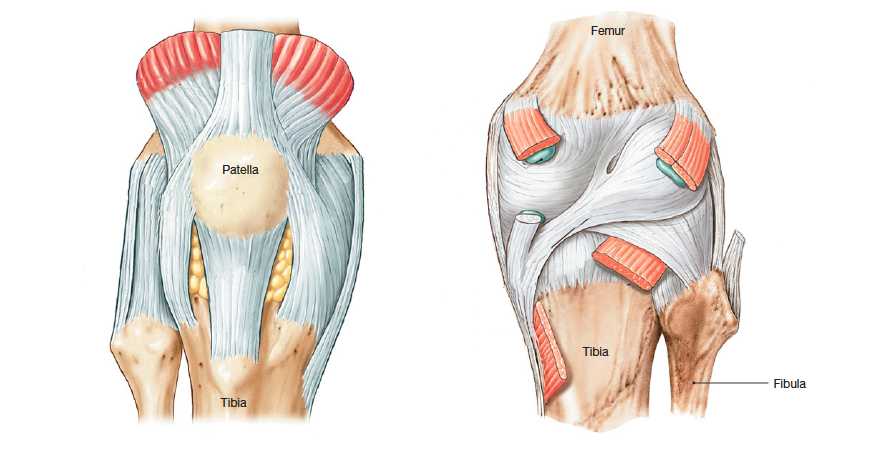
\includegraphics[width=0.8\textwidth]{figures/knae_anatomi}
\caption{Knæets anatomiske opbygning samt knæets forreste og bagerste korsbånd. \citep{aaos2014}.}
\label{fig:knae_anatomi}
\end{figure} 

\noindent
Ud over de tre separate ledforbindelser stabiliseres knæet af syv ledbånd. Ét af de syv ledbånd er patellarsenen, som er ansvarlig under extension af knæet. Derudover strækker to ledbånd sig mellem femur, tibia og fibia, hvilket er med til at styrke knæleddets overflade posteriort. 
Inde i ledkapslen befinder det forreste korsbånd, Anterior Cruciate Ligament (ACL), og det bagerste korsbånd, Posteior cruciate ligament (PCL), sig. Disse har til opgave at fastgøre indre knoglefremspring af tibia til knoglefremspringet på femur. 
Korsbåndene har til opgave at begrænse anteriore og posteriore bevægelser af femur og er med til at opretholde retningen af knoglefremspringene. 
Det tibiale kollaterale ligament forstærker den mediale flade af knæleddet, og det fibulære kollaterale ligament forstærker sidefladen. Disse ligamenter anvendes kun ved fuld ekstension af knæleddet \citep{martini2012}.

\subsection{Knæets funktion}
Ved gang aktiveres quadricepsmusklerne, der sidder anteriort på femur, og hasemusklerne, der sidder poseriort på femur. Nogle af disse muskler fremgår af \autoref{fig:laarmuskler}. Quadricepsmusklerne består af rectus femoris, vastus intermedius, vastus medialis og vastus lateralis. 
Hasemusklerne består af biceps femoris, semitendinosus og semimembranosus. 
Ved bevægelse foretager quadriceps- eller hasemusklerne ekstension eller fleksion, hvorved de fungerer som hinandens agonister eller antagonister under bevægelse \citep{martini2012}. 

\begin{figure} [H]
\centering
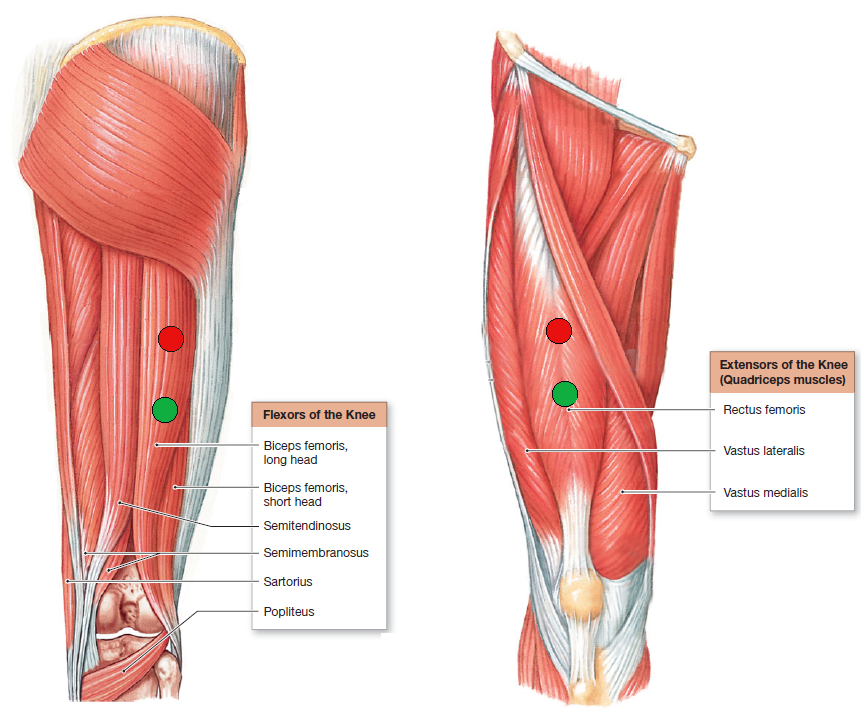
\includegraphics[width=0.9\textwidth]{figures/laarmuskler}
\caption{Viser rectus femoris, vastus lateris, biceps femoris, semimembranosus og patella  \citep{martini2012}.}
\label{fig:knaet}
\end{figure} 


Som tidligere nævnt anvendes hofte, knæ og ankler under gang. Udover disse led er kropsposituren og sving af leddene afgørende for gangfunktionen. Det fremgår af \autoref{fig:knaet}, hvordan de forskellige led udfører fleksion, ekstension og ændres fra ekstension til neutral bevægelse under gang \citep{martini2012}.

\subsubsection{Knæets funktion under en squat-øvelse} \label{sec:knaeled_squat}
% mere om, at det kun er lårets muskulatur, der benyttes under squat
Den dynamiske squat-øvelse er en udbredt træningsøvelse, som kræver styrke i flere muskelregioner. Squat aktiverer primært hofte-, lår- og rygmuskulaturen, som alle er primære muskler under gang, løb, spring og løft. Herudover anvendes squat som et redskab til rehabilitering af knæet, hvilket skyldes den måde, som knæet belastes under squat \citep{escamilla2001}. 

Knæets funktion for bøjningen af benet kan dermed ses ved udførelse af en squat-øvelse. En squat-øvelse udføres ved at stå i en oprejst position med knæ og hofte fuldt udstrakt. Herefter udføres en squat-øvelse i en kontinuerlig bevægelse, indtil den ønskede dybde nåes, hvorefter der udføres en kontinuerlig bevægelse tilbage til oprejst position \citep{escamilla2001}. En illustation af en squat-øvelse ses på \autoref{fig:squat}.

\begin{figure}[H]
\centering
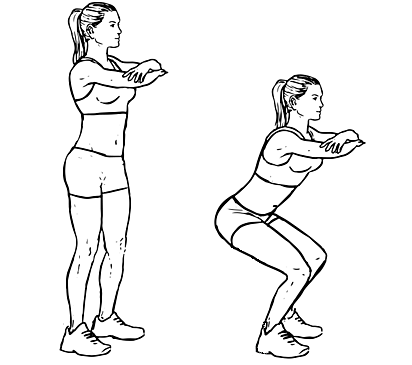
\includegraphics[width=0.5\textwidth]{figures/squat.png}
\caption{En illustration af udførelse af en halv squat-øvelse. Til venstre ses udgangspositionen, og til højre ses en halv squat-øvelse \citep{squat2015}.}
\label{fig:squat}
\end{figure}

\noindent 
Squat-øvelser kan udføres med varierende fleksion af knæet. De mest anvendte varianter af øvelsen er halv eller fuld squat. En halv squat-øvelse udføres indtil lårene er parallelle med jorden, hvilket svarer til en fleksion af knæet fra omkring $90-180^{\circ}$. En fuld squat-øvelse udføres indtil det posteriore del af låret og læggen kommer i kontakt med hinanden. Den fulde squat-øvelse anbefales mere trænede personer, hvorfor den halve squat-øvelse typisk er foretrukket til genoptræning af knæet \citep{escamilla2001}.

Ved udførelse af en squat-øvelse aktiveres blandt andet musklen rectus femoris. Aktiviteten i rectus femoris, og de resterende quadricepsmuskler, er størst ved $90-100^{\circ}$ vinkel af knæleddet \citep{schoenfeld2010}. 
Fra udgangspositionen for squat-øvelsen, der illustreres på \autoref{fig:squat}, befinder personen i en oprejst posistion med en vinkel på $180^{\circ}$ over knæet. Ved udførelse af en squat-øvelse vil muskelaktiviteten i rectus femoris være progressivt stigende indtil en vinkel over knæet på $90-100^{\circ}$ opnås. Idet der returneres til udgangspositionen, vil muskelaktiviteten være progressivt faldende \citep{escamilla2001}. 

%Biceps femoris aktiveres ved en $45^{\circ}$ fleksion af knæleddet, mens rectus femoris aktiveres ved en $80-90^{\circ}$ fleksion, hvorefter aktiviteten i musklerne er konsistent \citep{schoenfeld2010}. 


%Under en squat-øvelse aktiveres vastus intermedius, vastus medialis samt vastus lateris mere, da disse muskler er én ledmuskel, end rectus femoris der er en to-ledsmuskel \fxnote{hvorfor aktiveres én-ledsmuskler mere end to-ledsmuskler - jeg kan ikke finde det med hasemusklerne i den kilde der står til afsnittet?}.
%der er forbundet mellem femur, tibia og patella. Knæet har fire ledbånd. To af disse er side-ligamenterne, der sidder omkring knæleddet. De resterende to er korsbåndene, der sidder på skrå inden i knæet.
%Knæet fire ledbånd sikrer stabilisering af knæet og sørger for at knoglerne bevæger sig rigtigt.  Det er knæleddet, der gør det muligt for kroppen at kunne udføre aktiviteter som at kunne gå, løbe, og eksempelvis squatte. Ved gang aktiveres både quadriceps musklerne (rectus femoris, vastus intermedius, vastus medialis, vastus lateralis) der sidder anteriort for låret samt hamstring musklerne (biceps femoris, semitendinosus, Semimembranosus), der sidder posteriort for låret og kontraherer med quadriceps musklerne. 


\chapter{Problemformulering}

%-----------------------System udvikling-------------------------



%\section
Her skal der stå en mega nice introduktion til projektet som kan motivere læseren til at læse 100 siders rapport lavet af folk der ikke ved noget!
%% !TeX spellcheck = da_DK
\section
Min fantasi er sluppet op...\fixme{note til mig selv: køb noget mere fantasi}
%% !TeX spellcheck = da_DK
\section tralalalalala

tekst
 

%\printbibliography
\end{document}
